\documentclass{extbook}[14pt]
\usepackage{multicol, enumerate, enumitem, hyperref, color, soul, setspace, parskip, fancyhdr, amssymb, amsthm, amsmath, latexsym, units, mathtools}
\everymath{\displaystyle}
\usepackage[headsep=0.5cm,headheight=0cm, left=1 in,right= 1 in,top= 1 in,bottom= 1 in]{geometry}
\usepackage{dashrule}  % Package to use the command below to create lines between items
\newcommand{\litem}[1]{\item #1

\rule{\textwidth}{0.4pt}}
\pagestyle{fancy}
\lhead{}
\chead{Answer Key for Makeup Progress Quiz 3 Version A}
\rhead{}
\lfoot{1648-1753}
\cfoot{}
\rfoot{Summer C 2021}
\begin{document}
\textbf{This key should allow you to understand why you choose the option you did (beyond just getting a question right or wrong). \href{https://xronos.clas.ufl.edu/mac1105spring2020/courseDescriptionAndMisc/Exams/LearningFromResults}{More instructions on how to use this key can be found here}.}

\textbf{If you have a suggestion to make the keys better, \href{https://forms.gle/CZkbZmPbC9XALEE88}{please fill out the short survey here}.}

\textit{Note: This key is auto-generated and may contain issues and/or errors. The keys are reviewed after each exam to ensure grading is done accurately. If there are issues (like duplicate options), they are noted in the offline gradebook. The keys are a work-in-progress to give students as many resources to improve as possible.}

\rule{\textwidth}{0.4pt}

\begin{enumerate}\litem{
Construct the lowest-degree polynomial given the zeros below. Then, choose the intervals that contain the coefficients of the polynomial in the form $x^3+bx^2+cx+d$.
\[ 3 - 2 i \text{ and } -3 \]The solution is \( x^{3} -3 x^{2} -5 x + 39 \), which is option D.\begin{enumerate}[label=\Alph*.]
\item \( b \in [1.1, 4], c \in [-5.1, -3.6], \text{ and } d \in [-40, -32] \)

$x^{3} +3 x^{2} -5 x -39$, which corresponds to multiplying out $(x-(3 - 2 i))(x-(3 + 2 i))(x -3)$.
\item \( b \in [-0.4, 2], c \in [-2.9, 0.1], \text{ and } d \in [-9, -4] \)

$x^{3} + x^{2} -9$, which corresponds to multiplying out $(x -3)(x + 3)$.
\item \( b \in [-0.4, 2], c \in [3.2, 8.7], \text{ and } d \in [4, 7] \)

$x^{3} + x^{2} +5 x + 6$, which corresponds to multiplying out $(x + 2)(x + 3)$.
\item \( b \in [-6.7, -1], c \in [-5.1, -3.6], \text{ and } d \in [36, 41] \)

* $x^{3} -3 x^{2} -5 x + 39$, which is the correct option.
\item \( \text{None of the above.} \)

This corresponds to making an unanticipated error or not understanding how to use nonreal complex numbers to create the lowest-degree polynomial. If you chose this and are not sure what you did wrong, please contact the coordinator for help.
\end{enumerate}

\textbf{General Comment:} Remember that the conjugate of $a+bi$ is $a-bi$. Since these zeros always come in pairs, we need to multiply out $(x-(3 - 2 i))(x-(3 + 2 i))(x-(-3))$.
}
\litem{
Describe the end behavior of the polynomial below.
\[ f(x) = 2(x - 9)^{3}(x + 9)^{8}(x - 7)^{3}(x + 7)^{5} \]The solution is the graph below, which is option D.
    \begin{center}
        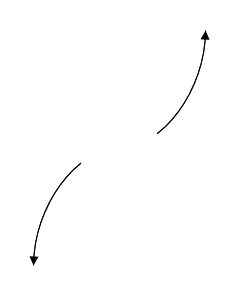
\includegraphics[width=0.3\textwidth]{../Figures/polyEndBehaviorDA.png}
    \end{center}\begin{enumerate}[label=\Alph*.]
\begin{multicols}{2}
\item 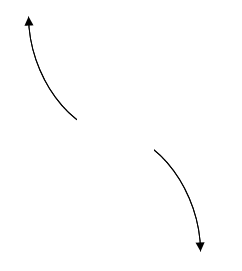
\includegraphics[width = 0.3\textwidth]{../Figures/polyEndBehaviorAA.png}
\item 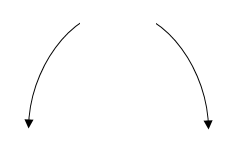
\includegraphics[width = 0.3\textwidth]{../Figures/polyEndBehaviorBA.png}
\item 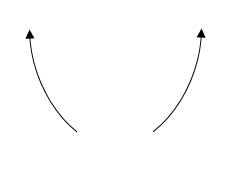
\includegraphics[width = 0.3\textwidth]{../Figures/polyEndBehaviorCA.png}
\item 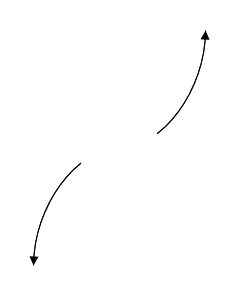
\includegraphics[width = 0.3\textwidth]{../Figures/polyEndBehaviorDA.png}
\end{multicols}\item None of the above.\end{enumerate}
\textbf{General Comment:} Remember that end behavior is determined by the leading coefficient AND whether the \textbf{sum} of the multiplicities is positive or negative.
}
\litem{
Describe the end behavior of the polynomial below.
\[ f(x) = -4(x - 2)^{5}(x + 2)^{10}(x - 3)^{5}(x + 3)^{6} \]The solution is the graph below, which is option B.
    \begin{center}
        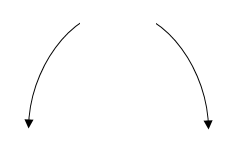
\includegraphics[width=0.3\textwidth]{../Figures/polyEndBehaviorCopyBA.png}
    \end{center}\begin{enumerate}[label=\Alph*.]
\begin{multicols}{2}
\item 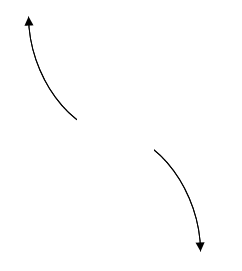
\includegraphics[width = 0.3\textwidth]{../Figures/polyEndBehaviorCopyAA.png}
\item 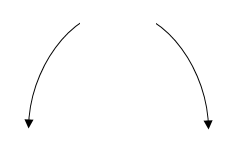
\includegraphics[width = 0.3\textwidth]{../Figures/polyEndBehaviorCopyBA.png}
\item 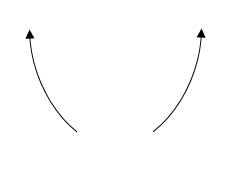
\includegraphics[width = 0.3\textwidth]{../Figures/polyEndBehaviorCopyCA.png}
\item 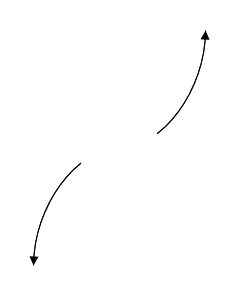
\includegraphics[width = 0.3\textwidth]{../Figures/polyEndBehaviorCopyDA.png}
\end{multicols}\item None of the above.\end{enumerate}
\textbf{General Comment:} Remember that end behavior is determined by the leading coefficient AND whether the \textbf{sum} of the multiplicities is positive or negative.
}
\litem{
Construct the lowest-degree polynomial given the zeros below. Then, choose the intervals that contain the coefficients of the polynomial in the form $ax^3+bx^2+cx+d$.
\[ -6, \frac{-3}{4}, \text{ and } \frac{7}{2} \]The solution is \( 8x^{3} +26 x^{2} -153 x -126 \), which is option C.\begin{enumerate}[label=\Alph*.]
\item \( a \in [3, 10], b \in [-75, -66], c \in [108, 118], \text{ and } d \in [125, 128] \)

$8x^{3} -70 x^{2} +111 x + 126$, which corresponds to multiplying out $(x -6)(4x + 3)(2x -7)$.
\item \( a \in [3, 10], b \in [-26, -24], c \in [-154, -145], \text{ and } d \in [125, 128] \)

$8x^{3} -26 x^{2} -153 x + 126$, which corresponds to multiplying out $(x -6)(4x -3)(2x + 7)$.
\item \( a \in [3, 10], b \in [23, 33], c \in [-154, -145], \text{ and } d \in [-130, -119] \)

* $8x^{3} +26 x^{2} -153 x -126$, which is the correct option.
\item \( a \in [3, 10], b \in [-89, -77], c \in [222, 233], \text{ and } d \in [-130, -119] \)

$8x^{3} -82 x^{2} +225 x -126$, which corresponds to multiplying out $(x -6)(4x -3)(2x -7)$.
\item \( a \in [3, 10], b \in [23, 33], c \in [-154, -145], \text{ and } d \in [125, 128] \)

$8x^{3} +26 x^{2} -153 x + 126$, which corresponds to multiplying everything correctly except the constant term.
\end{enumerate}

\textbf{General Comment:} To construct the lowest-degree polynomial, you want to multiply out $(x + 6)(4x + 3)(2x -7)$
}
\litem{
Describe the zero behavior of the zero $x = 3$ of the polynomial below.
\[ f(x) = 6(x - 3)^{4}(x + 3)^{9}(x + 7)^{4}(x - 7)^{8} \]The solution is the graph below, which is option C.
    \begin{center}
        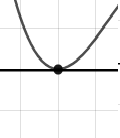
\includegraphics[width=0.3\textwidth]{../Figures/polyZeroBehaviorCA.png}
    \end{center}\begin{enumerate}[label=\Alph*.]
\begin{multicols}{2}
\item 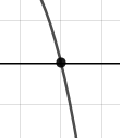
\includegraphics[width = 0.3\textwidth]{../Figures/polyZeroBehaviorAA.png}
\item 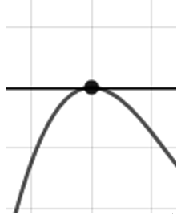
\includegraphics[width = 0.3\textwidth]{../Figures/polyZeroBehaviorBA.png}
\item 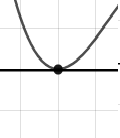
\includegraphics[width = 0.3\textwidth]{../Figures/polyZeroBehaviorCA.png}
\item 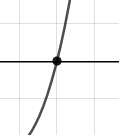
\includegraphics[width = 0.3\textwidth]{../Figures/polyZeroBehaviorDA.png}
\end{multicols}\item None of the above.\end{enumerate}
\textbf{General Comment:} You will need to sketch the entire graph, then zoom in on the zero the question asks about.
}
\litem{
Which of the following equations \textit{could} be of the graph presented below?

\begin{center}
    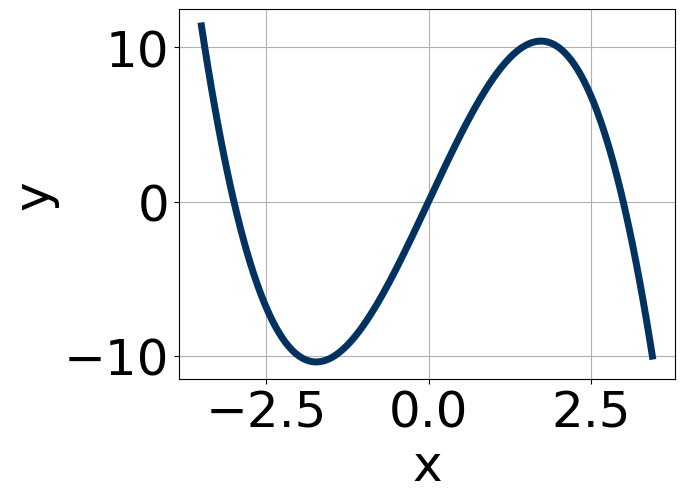
\includegraphics[width=0.5\textwidth]{../Figures/polyGraphToFunctionA.png}
\end{center}


The solution is \( -14x^{11} (x - 3)^{5} (x + 3)^{9} \), which is option C.\begin{enumerate}[label=\Alph*.]
\item \( 5x^{5} (x - 3)^{10} (x + 3)^{5} \)

The factor $(x - 3)$ should have an odd power and the leading coefficient should be the opposite sign.
\item \( -7x^{9} (x - 3)^{4} (x + 3)^{9} \)

The factor $3$ should have been an odd power.
\item \( -14x^{11} (x - 3)^{5} (x + 3)^{9} \)

* This is the correct option.
\item \( -18x^{9} (x - 3)^{4} (x + 3)^{8} \)

The factors $3$ and $-3$ have have been odd power.
\item \( 17x^{7} (x - 3)^{5} (x + 3)^{5} \)

This corresponds to the leading coefficient being the opposite value than it should be.
\end{enumerate}

\textbf{General Comment:} General Comments: Draw the x-axis to determine which zeros are touching (and so have even multiplicity) or cross (and have odd multiplicity).
}
\litem{
Construct the lowest-degree polynomial given the zeros below. Then, choose the intervals that contain the coefficients of the polynomial in the form $x^3+bx^2+cx+d$.
\[ -2 - 5 i \text{ and } 3 \]The solution is \( x^{3} + x^{2} +17 x -87 \), which is option A.\begin{enumerate}[label=\Alph*.]
\item \( b \in [0.2, 3.8], c \in [16.8, 19.7], \text{ and } d \in [-92, -81] \)

* $x^{3} + x^{2} +17 x -87$, which is the correct option.
\item \( b \in [0.2, 3.8], c \in [-3.5, 0.3], \text{ and } d \in [-9, -3] \)

$x^{3} + x^{2} -x -6$, which corresponds to multiplying out $(x + 2)(x -3)$.
\item \( b \in [-4.5, 0.5], c \in [16.8, 19.7], \text{ and } d \in [86, 92] \)

$x^{3} -1 x^{2} +17 x + 87$, which corresponds to multiplying out $(x-(-2 - 5 i))(x-(-2 + 5 i))(x + 3)$.
\item \( b \in [0.2, 3.8], c \in [1.8, 4.3], \text{ and } d \in [-18, -11] \)

$x^{3} + x^{2} +2 x -15$, which corresponds to multiplying out $(x + 5)(x -3)$.
\item \( \text{None of the above.} \)

This corresponds to making an unanticipated error or not understanding how to use nonreal complex numbers to create the lowest-degree polynomial. If you chose this and are not sure what you did wrong, please contact the coordinator for help.
\end{enumerate}

\textbf{General Comment:} Remember that the conjugate of $a+bi$ is $a-bi$. Since these zeros always come in pairs, we need to multiply out $(x-(-2 - 5 i))(x-(-2 + 5 i))(x-(3))$.
}
\litem{
Describe the zero behavior of the zero $x = 5$ of the polynomial below.
\[ f(x) = -9(x - 6)^{11}(x + 6)^{9}(x - 5)^{7}(x + 5)^{6} \]The solution is the graph below, which is option D.
    \begin{center}
        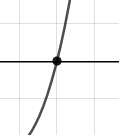
\includegraphics[width=0.3\textwidth]{../Figures/polyZeroBehaviorCopyDA.png}
    \end{center}\begin{enumerate}[label=\Alph*.]
\begin{multicols}{2}
\item 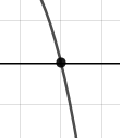
\includegraphics[width = 0.3\textwidth]{../Figures/polyZeroBehaviorCopyAA.png}
\item 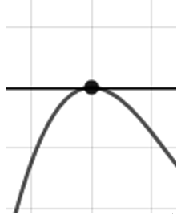
\includegraphics[width = 0.3\textwidth]{../Figures/polyZeroBehaviorCopyBA.png}
\item 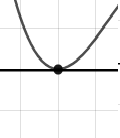
\includegraphics[width = 0.3\textwidth]{../Figures/polyZeroBehaviorCopyCA.png}
\item 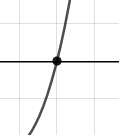
\includegraphics[width = 0.3\textwidth]{../Figures/polyZeroBehaviorCopyDA.png}
\end{multicols}\item None of the above.\end{enumerate}
\textbf{General Comment:} You will need to sketch the entire graph, then zoom in on the zero the question asks about.
}
\litem{
Construct the lowest-degree polynomial given the zeros below. Then, choose the intervals that contain the coefficients of the polynomial in the form $ax^3+bx^2+cx+d$.
\[ \frac{5}{3}, 7, \text{ and } \frac{-7}{5} \]The solution is \( 15x^{3} -109 x^{2} -7 x + 245 \), which is option B.\begin{enumerate}[label=\Alph*.]
\item \( a \in [13, 24], b \in [143, 153], c \in [348, 358], \text{ and } d \in [239, 253] \)

$15x^{3} +151 x^{2} +357 x + 245$, which corresponds to multiplying out $(3x + 5)(x + 7)(5x + 7)$.
\item \( a \in [13, 24], b \in [-110, -101], c \in [-10, -4], \text{ and } d \in [239, 253] \)

* $15x^{3} -109 x^{2} -7 x + 245$, which is the correct option.
\item \( a \in [13, 24], b \in [-110, -101], c \in [-10, -4], \text{ and } d \in [-247, -238] \)

$15x^{3} -109 x^{2} -7 x -245$, which corresponds to multiplying everything correctly except the constant term.
\item \( a \in [13, 24], b \in [106, 114], c \in [-10, -4], \text{ and } d \in [-247, -238] \)

$15x^{3} +109 x^{2} -7 x -245$, which corresponds to multiplying out $(3x + 5)(x + 7)(5x -7)$.
\item \( a \in [13, 24], b \in [-60, -56], c \in [-287, -277], \text{ and } d \in [-247, -238] \)

$15x^{3} -59 x^{2} -287 x -245$, which corresponds to multiplying out $(3x + 5)(x -7)(5x + 7)$.
\end{enumerate}

\textbf{General Comment:} To construct the lowest-degree polynomial, you want to multiply out $(3x -5)(x -7)(5x + 7)$
}
\litem{
Which of the following equations \textit{could} be of the graph presented below?

\begin{center}
    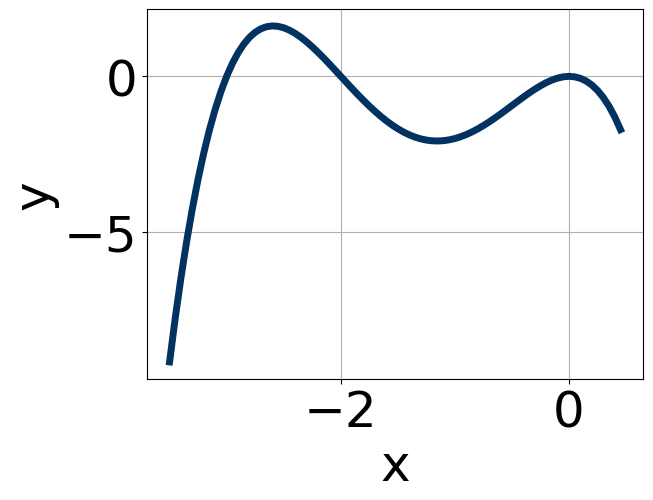
\includegraphics[width=0.5\textwidth]{../Figures/polyGraphToFunctionCopyA.png}
\end{center}


The solution is \( -18x^{6} (x + 3)^{11} (x + 2)^{9} \), which is option E.\begin{enumerate}[label=\Alph*.]
\item \( 9x^{4} (x + 3)^{7} (x + 2)^{11} \)

This corresponds to the leading coefficient being the opposite value than it should be.
\item \( -20x^{10} (x + 3)^{10} (x + 2)^{11} \)

The factor $(x + 3)$ should have an odd power.
\item \( 14x^{4} (x + 3)^{9} (x + 2)^{8} \)

The factor $(x + 2)$ should have an odd power and the leading coefficient should be the opposite sign.
\item \( -13x^{9} (x + 3)^{6} (x + 2)^{9} \)

The factor $0$ should have an even power and the factor $-3$ should have an odd power.
\item \( -18x^{6} (x + 3)^{11} (x + 2)^{9} \)

* This is the correct option.
\end{enumerate}

\textbf{General Comment:} General Comments: Draw the x-axis to determine which zeros are touching (and so have even multiplicity) or cross (and have odd multiplicity).
}
\end{enumerate}

\end{document}